\chapter{Polymerase Chain Reaction (PCR)}

\vspace{0.6cm}


\section{Sommario}

\subsection{Scopo}

In questa esperienza di laboratorio eseguiamo la PCR, una tecnica che fa uso della
DNA polimerasi con lo scopo di amplificare un frammento di DNA ed ottenere così un
ampio numero di copie.\\

\subsection{Cenni teorici}

La PCR è composta da una serie di cicli (con temperature e tempistiche differenti)
che si svolgono in uno specifico macchinario chiamato \textbf{termociclatore},
che permette di eseguire questi cicli in maniera automatica.
Per effettuare la PCR inoltre prepareremo un gel di agarosio 0,8\%
su cui avverrà la corsa elettroforetica.

\subsection{Materiali utilizzati}

\begin{itemize}
	\item Eppendorf
	\item Micropipette
	\item Forno microonde
	\item Vaschetta per Elettroforesi
	\item Lampada UV
	\item Beuta
\end{itemize}

\subsection{Soluzioni utilizzate}
\begin{itemize}
	\item H$_2$O sterile
	\item Buffer TAQ 10X
	\item MgCl$_2$
	\item Primer FOR
	\item Primer REV
	\item DNA plasmidico contenente l'inserto da amplificare (GPR3), circa 1000bp
	\item TAQ polimerasi
\end{itemize}

\section{Procedimento}

\subsection{Preparazione PCR}

Prendiamo una eppendorf da 250 $\mu$l in cui bisogna aggiungere (Attenzione a non contaminare):
\begin{itemize}
	\item 12 $\mu$l H2O sterile
	\item 2 $\mu$l buffer TAQ (10X)
	\item 1 $\mu$l MgCl2 (50mM)
	\item 1 $\mu$l Primer FOR (25 $\mu$M)
	\item 1 $\mu$l Primer REV (25 $\mu$M)
	\item 1 $\mu$l dNTPs (10 mM)
	\item 1 $\mu$l DNA plasmidico contenente l’inserto da amplificare (GPR3), circa 1000 bp
	\item 1 $\mu$l TAQ polimerasi
\end{itemize}

Totale 20 $\mu$l\\

Il mix ottenuto nella eppendorf
viene inserito nel termociclatore, i cui cocli sono specificati nella figura \ref{cicli_termociclatore}.
\begin{figure}[htbp]
	\centering
	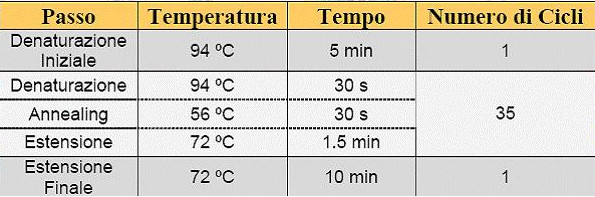
\includegraphics[width=80mm]{./immagini/cicli_termociclatore.jpg}
	\caption{Cicli termociclatore}
	\label{cicli_termociclatore}
\end{figure}

\subsection{Preparazione gel di agarosio 0,8\%}

Passiamo alla preparazione del gel di Agarosio 0,8\% per la corsa elettroforetica.
Pesiamo le seguenti quantità per un gel allo 0,8\% in una beuta:

\begin{itemize}
	\item 0,6 g  di agarosio
	\item 1,6  ml TAE 50X
	\item 78,4 ml H2O
\end{itemize}

Totale 80 ml
\begin{enumerate}
\item Scaldare nel forno a microonde la beuta con i componenti facendo attenzione a
non portare ad ebollizione, mescolando ogni tanto per sciogliere bene.
\item Aggiungere 5 $\mu$l di SyberSafe.
\item Mescolare e versare nell’apposita vaschetta
usando il pettine per creare i pozzetti.
\item A gel solidificato togliere il pettine e
aggiungere 250 ml di buffer di corsa (TAE 1X).

\item Preparato il gel nella camera per l’elettroforesi caricare nei pozzetti la
soluzione preparata in precedenza dopo che il termociclatore ha terminato il
lavoro.
\item Avviare la corsa elettroforetica.

\item Finita la corsa elettroforetica, con l’ausilio di una lampada UV, osservare il
risultato ottenuto.

\end{enumerate}


\section{Risultati e Conclusioni}

Controllando la fluorescenza possiamo capire l'efficacia della replicazione
ottenuta. Confrontando il pozzetto caricato da noi con un secondo pozzetto
dove è presente un marker possiamo capire se la PCR ha replicato il nostro
frammento di DNA o anche altri frammenti aspecifici.

\begin{figure}[htbp]
	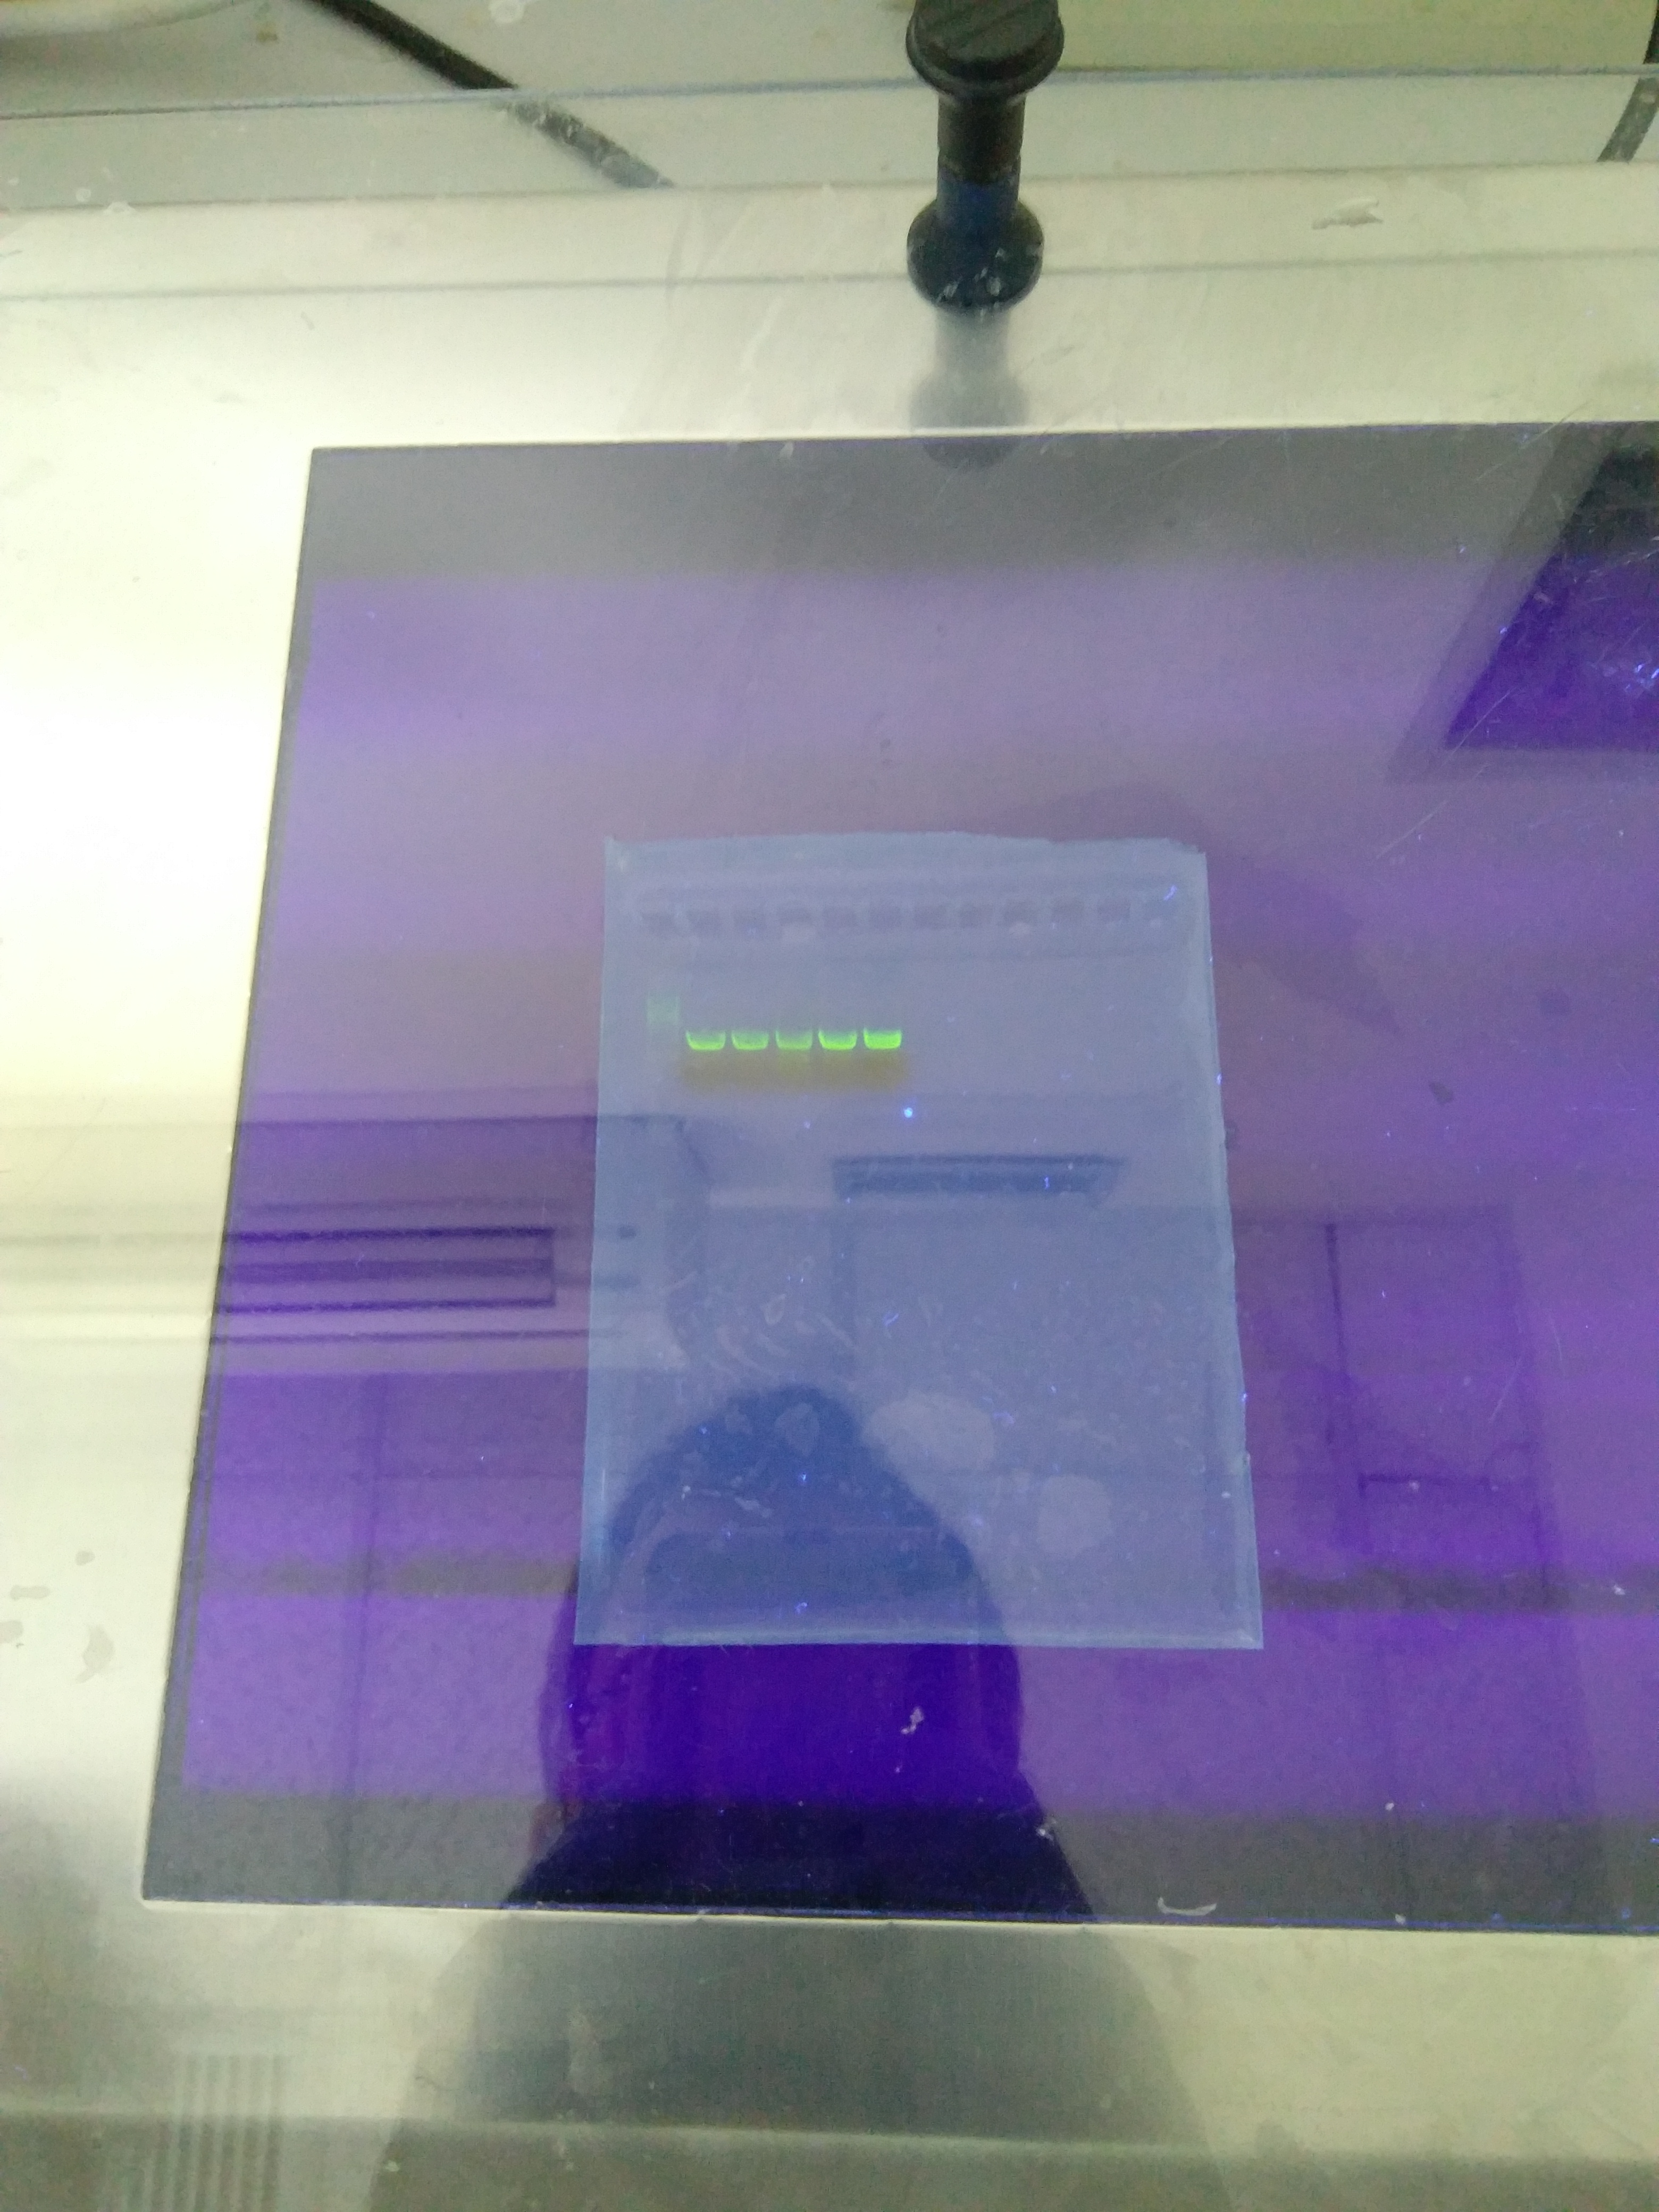
\includegraphics[width=50mm]{./immagini/risultato_pcr.jpg}
	\caption{Risultato della PCR}
	\label{risultato_pcr}
\end{figure}
